\section{Modelling results and analysis}
\label{S:results}
Four models are developed and compared in this section: a simple binary choice model as a ground for comparison of the performance of survival models, a traditional CPH model with linear log-partial hazard function, a deep neural network-based CPH function (DCPH1), and a deep neural network-based CPH function empowered by RreliefF (DCPH2).

\subsection{Model performance}
Applying VIF before developing the models is essential to remove highly correlated variables, as models consisting of them fail to converge because of non-invertibility of singular matrices. Models are developed over a training dataset, consisting of 80\% of the data, and evaluated on a test dataset, both of which selected randomly. To measure the goodness of fit of the models, \textit{Concordance Index (C-index)} is used as the global index for comparing survival times. C-index is defined as the fraction of pairs of observations, in which the observation with higher predicted risk of starting a cross has shorter waiting time.
\subsubsection{Binary Choice model}
As a base case for comparison of survival models' performance to other approaches, a binary choice model is developed. For every 100 milliseconds interval (the interval captured by the VR), a participant is faced with two choices: whether to initiate a cross or not. The independent variables used to develop the model are all the covariates used for developing survival models, plus a variable representing the time passed since the start of the experiment. The latter variable is needed to distinguish the instances of a single experiment from each other. Thus, a great advantage of using CPH partial hazard function, i.e. estimation of the effect of covariates regardless of the time the pedestrian has spent on the sidewalk, is missing. Applying all the data cleaning procedures and model evaluation metrics in the same way as the survival models, a C-index of 0.58 over the training set, and 0.56 over the test set is achieved.
\subsubsection{Cox Proportional Hazards model}
 After removing highly correlated variables, CPH model is developed using Python's lifeline package~\citep{cameron_davidson_pilon_2020_4002777} starting with all the remained variables and iteratively removing insignificant variables. Developing a CPH model over the train dataset using 10-fold cross validation, a C-Index of 0.57 is achieved on the test set. Details of the performance of CPH model are presented in \cref{tab:compare}.
\subsubsection{Deep CPH model (DCPH)}
After applying VIF to remove highly correlated variables, variables are ranked based on their importance according to their RReliefF importance weights, before training the network. Hyperparameter $n$ is introduced as the number of covariates to be used in training the network. Other hyperparameters include: number of hidden layers, number of nodes in hidden layers, learning rate and learning rate decay for optimization, whether to use batch normalization, and dropout layer and its rate. To find the best model, random search for optimizing hyperparameters is utilized~\citep{bergstra2012random}. In \cref{tab:hyper}, the optimum values for hyperparameters based on a 10-fold cross-validation over 100 epochs on training dataset are presented. 
\begin{table}[t]
\caption{Model parameters}
\centering
\begin{tabular}{|c|c|}
\hline
 \thead{\textbf{Parameter}} & \thead{\textbf{Value}} \\
\hline
     Number of Hidden Layers&3\\
     Number of Nodes in Hidden Layers&90 \\
     Batch Normalization&True\\
     Dropout Rate & 0.1\\
     Learning Rate& 0.001\\
     Learning Rate Decay& 0.001\\
     
     \hline
\end{tabular}
\label{tab:hyper}
\end{table}
Same test dataset as the one used for CPH is used again to evaluate the performance of the network over 100 epochs. Using a framework with $n=$19 top covariates as inputs, three hidden layers of 90 units each, batch normalization and a dropout rate of 0.1, a C-index of 0.64 in cross-validation and 0.62 for test set is achieved, showing an improvement of 5 percent compared to CPH.

To further assess the performance of the proposed framework, another neural-network based survival model is developed without incorporation of RreliefF and VIF (DCPH1). C-indices of all four models, along with the number of covariates incorporated in the models are presented in \cref{tab:compare}. It can be observed that in general survival models are performing better than simple binary choice models, with a slight improvement in linear CPH and greater improvements in DCPH2. Also, DCPH2 outperforms all the other models, with 5\% and 2\% improvement over Linear CPH and DCPH1, respectively. Comparing the number of covariates used, using DCPH2, the process of removing insignificant covariates and retraining the models to find the best combination of covariates manually is no longer required. Compared to DCPH1, DCPH2 results in a better C-index with less number of covariates, meaning a less computationally expensive prediction in DCPH2.
\begin{table}[t]
\caption{Comparing the performance of the models}
\centering
\begin{tabular}{|c|c|c|c|}
\hline
 \thead{\textbf{Model}} & \thead{\textbf{Number of}\\\textbf{covariates}} & \thead{\textbf{C-index:} \\ \textbf{Validation Set}} & \thead{\textbf{C-index:} \\ \textbf{Test Set}} \\
\hline
    Binary Choice & 11(+intercept)&0.59&0.57\\
     Linear CPH&10 &0.60&0.57\\
     DCPH1&21& 0.61 & 0.60 \\
     DCPH2&19 & \textbf{0.64} &\textbf{0.62}\\ 
     \hline
\end{tabular}
\label{tab:compare}
\end{table}
\subsection{Covariates and their effects}
\subsubsection{Binary Choice model}
\cref{tab:bc} shows the significant variables in the binary choice models. The large coefficient achieved for intercept, and the significance of elapsed time are the major differences in binary choice model's interpretation compared to the survival models. All the other significant variables and their effects are similar to results obtained by linear CPH (\cref{tab:cox}). A positive coefficient of variable shows the effect of that variable on increasing the tendency of the participant to start crossing, whereas a negative coefficient means contribution to the decision of not to cross. Two major issues remain with the binary choice model, aside from its accuracy. First, the requirement of the variable elapsed time since the start of the experiment, makes this approach dependent on knowing the time that pedestrian has already waited on the sidewalk. CPH based models, on the other hand, rely solely on the covariates on partial hazard model, and the time parameters are left to baseline hazard function. Second issue with binary choice model is the need for discretization of wait time, and relying on decisions of cross or not, rather than the continues approach of survival models. 
\begin{table}
\caption{Binary choice model results}
\footnotesize
    \centering
    
    \begin{tabular}{|ccc|}
    \hline
         \textbf{Variable}&\textbf{Coefficient}& \textbf{p-value}  \\
    \hline
         Intercept&-3.51 & $<$0.005\\
    \hline
         Elapsed Time&-3.06&$<$0.005\\
    \hline
         Traffic Density&-0.86&$<$0.005\\
    \hline 
         Age: 30-39&0.37&$<$0.005\\
     \hline
         Lane Width&-0.34   &$<$0.005\\
    \hline
    Main Mode: Active Modes&-0.29	&$<$0.005\\
    \hline
         Road Type: Two-way with Median&  0.26&$<$0.005\\
    \hline
        Main Mode: Car&	-0.21&$<$0.005\\
    
    \hline
         Previous VR Experience& 0.21	&$<$0.005\\
    \hline
         No Cars in the Household&  0.21	&$<$0.005\\
    \hline
         Age Over 50&-0.20&0.035\\
    \hline
         Gender: Female&-0.12&0.023\\
    
    \hline
    
    \end{tabular}
    
    \label{tab:bc}
\end{table}
\subsubsection{Cox Proportional Hazards model}
Covariates used for developing CPH are listed in \cref{tab:cox}, along with their coefficients, Hazard Ratios and P-Values as a measure of significance. P-Value of 0.1 (90\% confidence interval) is set as the threshold of significance for selecting the covariates. The third column of the table provides \textit{Hazard Ratio}, which is defined as the ratio of the hazard rates of two conditions of a covariate. A hazard ratio of 0.84 for binary covariate \textit{Age Over 50}, for instance, means that the hazard of a pedestrian older than 50, over the hazard of other pedestrians equals 0.84, implying lower probability of crossing (longer waiting times) for pedestrians aged over 50. Hazard ratio is calculated as the exponential of coefficients in the second column. In other words, a higher coefficient, implies higher hazard ratio, and a hazard ratio greater than 1 (positive coefficient) means that the probability of a cross is higher for instances having greater values of that covariate, leading to shorter waiting times. Based on the results in \cref{tab:cox}, participants who walk to do their shoppings, have previous VR experience, aged between 30 and 39, or have no cars in the household wait shorter in our sample of collected data compared to their counterparts with different values for each of the mentioned covariates. Moreover, experiments on two-way roads with median take shorter wait time compared to two-way roads with no median as the baseline variable of this covariate. On the other hand, participants who indicated their main mode of travel as cars, are aged over 50, or are females, have longer wait times. In addition, experiments in higher traffic densities and higher lane widths makes pedestrians wait longer in our sample data.

Going deeper into the effects of covariates, it can be inferred that participants who tend to have the walking habits in their life-style, i.e. walk for doing their shops and have no cars in their households, feel more comfortable crossing the streets, and have shorter waiting times. On the other hand, participants who use cars as their main mode of transportation, are expected to be less familiar with the crossing conditions and have to wait longer before initiating a cross. Considering gender and age covariates, it can be observed that females in our sample size waited longer before crossing, which is in line with some of the previous studies in the literature. The eldest age group of participants, who are over the age of 50, also tend to spend more time on the sidewalk before crossing the street. One the other hand, participants in the second youngest age group wait on the sidewalk for shorter times compared to the baseline category for age: 40 to 49. The developed model does not consider age category of between 18 and 29 as a significant variable, which can be resulted by the high heterogeneity of the participants in this age category.
Regarding variables related to geometry of the road, participants tend to wait longer before crossings roads with larger lane width. Significance of this variable can lead to the promotion of larger sizes for sidewalks and narrower lane widths. As stated earlier, out of the three road types, two-way roads with no median are settled as the baseline category of road type. Compared to the baseline category, medians help pedestrians cross with shorter waiting times.
Other significant covariate set by the scenario is traffic density on road, for which higher values lead to longer waiting times by the participants, due to the time required to find the appropriate safe gaps for crossing.
Finally, having previous VR experience helps participants of our experiment cross in shorter times. Despite having a 5-minute familiarization session with the equipment and environment before the experiments, it seems that further tutorials can be helpful to participants with no prior VR experience in future studies.

An interesting observation on the results of CPH is the insignificance of the level of traffic automation status, as well as other scenario-related variables, on participants' wait time. As different pedestrian's behaviours was expected for different scenarios, it can be inferred that linear CPH is incapable of capturing complex relationships among the covariates and wait time.   
\begin{table}
\caption{Multivariate proportional hazard model results}
\footnotesize
    \centering
    
    \begin{tabular}{|cccc|}
    \hline
         \textbf{Variable}&\textbf{Coefficient}&\textbf{Hazard Ratio}& \textbf{p-value}  \\
    \hline
         Traffic Density&-0.83& 0.43&$<$0.005\\
    \hline 
         Age: 30-39&0.32&1.38&$<$0.005\\
    \hline
         Lane Width&-0.31   &   0.73&$<$0.005\\
    \hline
         Road Type: Two-way with Median&0.22&  1.24&$<$0.005\\
    \hline
         Walk to Shopping&0.18&1.20&$<$0.005\\
    
    \hline
         Age Over 50&-0.17& 0.84&0.06\\
    
    \hline
         Previous VR Experience&0.14& 1.15&$<$0.005\\
    
    
    \hline
         No Cars in the Household&0.14&  1.15&$<$0.03\\
    \hline
         Gender: Female&-0.13& 0.87&0.01\\
    \hline
         Main Mode: Car&-0.12 & 0.88&0.03\\
    \hline
    
    
    \end{tabular}
    
    \label{tab:cox}
\end{table}

\subsubsection{Deep CPH (DCPH) model}
SHAP in its core, estimates the contribution of covariates to the waiting time for each instance separately. Each SHAP value, corresponds to the contribution of the covariate to log-partial hazard values, compared to when the covariate has a baseline value, called \textit{background} value in SHAP terminology~\citep{molnar2019interpretable}. Default baseline values for a covariate in the original paper are set to be equal to the average value of that covariate. In this study, we used the default values for continues covariates. However, the question arises for binary variables, in which having a real number value does not have a meaningful interpretation outside of the model. To address this issue, we set the baseline value for binary variables to zero, thus comparing the contribution of each binary covariate of an instance to cases where the same covariate has a value of zero. By doing so, SHAP value of a covariate in instances that the value of that covariate is zero is not calculated and contribution of a covariate is assessed based on SHAP values of the covariate in other instances. In \cref{fig:shap}, SHAP Values for the covariates for all the instances are depicted. Feature values are the values that covariates take, represented in the color. A dot in red means an instance with the higher than baseline value for that covariate, and blue means an instance with lower values in that covariate. As stated, the baseline value for binary covariates is set to zero. Thus, the instances with a value of zero in binary covariates are not taken into account for calculating the impact (blue dots on the central axis in \cref{fig:shap}).

To have a numerical understanding of SHAP values, average and standard deviation of SHAP values for all 19 covariates used in training the network, and over all instances, are presented in \cref{tab:sh}, sorted by their importance according to SHAP values. As a rule of thumb, we consider the overall contribution of a covariate interpretable, if it has a relatively uniform effect on a major part of instances. In other words, if for a covariate, the absolute mean of SHAP values is greater than the standard deviation of the SHAP values, over all instances, we call the effect of that covariate uniform. It should be noted that non-uniformity of SHAP values does not mean insignificance of that covariate. Non-uniformity reveals that the interpretability method used could not capture the complex non-linear multi-level relationship among covariates. Intuitively, a covariate has non-uniform SHAP values when it has a wide range of SHAP values, extending over negative and positive values, as in these cases, the effects can vary based on the instance. 

Looking into SHAP values in \cref{fig:shap}, it can be observed that unlike CPH that was not able to capture the effects, automation level covariates have generally a negative contribution to log-partial hazard, leading to longer waiting times. Relatively high mean and low standard deviation of fully automated and mixed traffic conditions in \cref{tab:sh} confirms the significant negative effect of these two covariates on log-partial hazard. As pedestrians feel more unfamiliar and concerned with cars with no drivers, the effects were expected, but could not be captured by linear CPH. By assuming that pedestrians have lower trust in AVs compared to human-driven vehicles, longer waiting time for pedestrians facing AVs in our experiments is aligned with the hypothesis made in~\citep{jayaraman2019pedestrian}, but contrasts their finding that a positive correlation exists between trust in AVs and average waiting time before cross. However, different participants' demographics and sample sizes, definition of trust, and different scenarios tested in the two studies need to be taken into account before driving to a conclusion.
\begin{table}
\caption{DCPH2 interpretability results, sorted by the absolute mean SHAP value}
\footnotesize
    \centering
    \begin{tabular}{|ccc|}
    \hline
    \textbf{Variable} &   \textbf{Mean SHAP Value} &  \textbf{std of SHAP Values} \\
    \hline
    Mixed Traffic Conditions & -0.535410 &  0.299655 \\
    \hline
    Previous VR Experience & 0.492931 &  0.193912\\
    \hline
    Fully Automated Conditions&-0.430101 &  0.272217\\
    \hline
    Walk to Work& 0.423793 &  0.260193 \\
    \hline
    Time: Night& 0.381095 &  0.202777 \\
    \hline
    Main Mode: Active Modes	&-0.372863 &  0.410266 \\
    \hline 
    Weather: Snowy&-0.232487 &  0.179340 \\
    \hline
    Age: 30 - 39	& 0.231225 &  0.263909 \\
    \hline
    Age Over 50&-0.224146 &  0.374447 \\
    \hline
    Main Mode: Car&-0.219562 &  0.288102 \\
    \hline
    Lane Width&-0.197134 &  0.174416 \\
    \hline
    Traffic Density&-0.189191 &  0.134376 \\
    \hline
    Age: 18 - 29	&-0.149895 &  0.262167 \\
    \hline
    More than 1 Car in the Household& 0.128925 &  0.308825 \\
    \hline
    Walk to Shopping&-0.072093 &  0.267495 \\
    \hline
    Gender: Female& 0.041379 &  0.296014 \\
    \hline
    Vehicle Arrival Rate& 0.041003 &  0.084269 \\
    \hline
    Road Type: One Way&-0.025349 &  0.201819 \\
    \hline
    Participant Owns a Driving License	&-0.009217 &  0.282812 \\
    \hline
    \end{tabular}
    \label{tab:sh}
\end{table}


Positive contribution captured for previous VR experience is in line with the results obtained in CPH, which confirms the necessity of stronger VR tutorials before experiments. Similar to CPH, wider lane width and higher traffic density both have negative effect on log-partial hazard, implying longer waiting times. Their mean and standard deviation confirm the uniformity of SHAP values for these two covariates. The effect of lane width is in line with~\citep{rasouli2017agreeing}, where authors, using real video data from urban and suburban roads, report pedestrians paying more attention before crossing wider streets. The reported effects of traffic parameters on pedestrian behaviour in previous studies also confirm the negative effect of traffic density on waiting time~\citep{schmidt2009pedestrians,ishaque2008behavioural}. Schmidt~\textit{et al.}~\cite{schmidt2009pedestrians}, for instance, suggest speed and density as important parameters for pedestrians crossing decision, with pedestrians using distance of the vehicles for making crossing decisions.
Six of the used covariates are relevant to walking habits: Walk to work and shopping, main transportation mode of cars and active modes, having driving licence and having more than 1 car in the house. Among them, only walking to work appears to be interpretable based on mean and standard deviation of SHAP values, which shows shorter waiting time for participants who indicated that they walk to commute to their works. Similar results are obtained in \citep{hamed2001analysis} with analysing wait time of pedestrians in divided and undivided streets. Based on their study, pedestrians owning cars have longer wait times due to their greater perception of risk. 
Environmental covariates, on the other hand, are added to the model and appear to have uniform effect. Results showed that participants crossing in simulated snowy scenarios, have longer wait times, which may be traced to poor sight distance. Previous studies confirm this observation, where bad weather conditions are associated with a negative effect on pedestrians' perception of speed, and being more conservative~\citep{rasouli2019autonomous,sun2015estimation,harrell1991factors}. On the other hand, in the night scenarios, participants tended to have shorter wait times, which is not consistent with the supposed poor sight distance in the simulation. Poor sight distance at nights has also been associated with riskier decisions ~\citep{rasouli2019autonomous}, which might justify the shorter wait times of pedestrians. However, in our study we solely focus on safe crossings and it is not clear whether we can assume crosses with shorter wait times more \textit{risky}. The contribution of night time to shorter wait time in our study may be due to the fact that in night scenarios simulated, unlike snowy simulated scenarios, the sight observed by participants was not limited and changes were only made to the color of the sky to project the mental effect of night. This can be addressed in future data collection campaigns. 
The effect of road type covariate did not appear to be interpretable over all instances, and vehicle arrival rate, although not one of CPH covariates, appeared to be one of the selected covariates by DCPH2, without captured uniform contribution for all instances. 

Interactions with other covariates may be investigated to further analyze the effects of covariates with non-uniform contributions. Numerous possible combinations can be defined and investigated. In this study, however, we limit our analysis to two-level combinations, and more complex combinations are left as a future direction. \cref{tab:int} shows the two-level interactive effect of the investigated covariates. All the provided combinations have appeared to be significant based on the values of the mean and standard deviation of their SHAP values. The first column represents the variable upon which the combination is conditioned, and the second column of the table shows the variable that its effect is investigated under the condition variable. To better understand the effect of age and gender, combined effects of some covariates conditioned upon three relevant covariates to age and gender are investigated. Gender is arguably one of the determining factors in explaining pedestrians' behaviour~\cite{rasouli2019autonomous,hamed2001analysis}. The differences in crossing behaviour of males and females are traced back to differences in motives~\citep{yagil2000beliefs}, attention to environment~\citep{tom2011gender}, and females being more cautious~\citep{holland2007effect}. However, this trend in general is not observed in our modelling results. Part of this inconsistency might be explained by the use of VR in our experiment, where details are not as elaborate as real life, risk involved is less and laws are not as strict as real streets. Interaction of gender with some other variables, however, suggest gender contribution to wait time in some scenarios: In mixed traffic conditions, females wait longer. The pattern exists in fully automated conditions, but the contribution is not uniform and thus we have not included it in the table. Among those participants whose main mode of transportation is their car, females appear to be more conservative. In one-way roads, females also tend to wait longer compared to men. Gender appeared to be insignificant in different weather conditions and times of the day. Results also show that having strong walking habits helps both younger and older age groups cross in shorter times. On the other hand, although participants of age over 50 wait longer in the presence of automated vehicles in the experiment, younger participants do not seem to be affected significantly by this factor. Similarly, among participants aged over 50, waiting in snowy weather takes longer. Similar trends occur for female participants, as a lack of walking habits, presence of AVs and snowy weather conditions make the wait times before cross take longer. Also among females, having an age of over 50 contributes to longer wait times. Generally, studies on the effect of age suggest elderly population are more cautious~\citep{sun2003modeling,harrell1991precautionary,hamed2001analysis}. Although age does not have a uniform contribution in our case, having an age of over 50 in poor sight distances, and for females, is shown to be a contributing factor.  Effects of walking habits, automation condition of the vehicles on the road, age and snowy weathers during night scenarios follow an expected pattern. When night scenario are accompanied by snowy weathers and thus poor sight distances, the waiting times before crosses are increased. Also, elderly people are behaving more conservatively in night scenarios as opposed to other age brackets in our experiment. Higher traffic densities and wider lane widths were both associated with longer wait times based on the single-level analysis in \cref{tab:sh}. However, having walking habits appear to be effective in decreasing the wait time among high density scenarios and wide lane width scenarios. Fully automated or mixed traffic conditions also contribute to longer waiting times, even among high traffic densities and wide lane width scenarios.
\begin{table}
\caption{DCPH2 interaction variables results}
\footnotesize
    \centering
    \begin{tabular}{|ccc|}
    \hline
    \textbf{Condition Variable} &   \textbf{Variable} &  \textbf{Mean SHAP Value} \\
    \hline
    Mixed Traffic Condition & \multirow{3}{*}{Gender: Female} &-0.100629 \\ Main Mode: Car& &-0.263754\\Road Type: One Way && -0.229365 \\
    \hline
    \hline
    \multirow{2}{*}{Age 18 - 29} & Walk to Work &  0.437002  \\
    &Main Mode: Car &  -0.377411\\
    \hline
    \hline
    \multirow{4}{*}{Age Over 50} & Walk to Work &  0.668556 \\
    
     & Weather: Snowy&  -0.377821 \\
    
    &Fully Automated Conditions &  -0.614000\\
    &Mixed Traffic Conditions &  -0.630974\\
    \hline
    \hline
    \multirow{5}{*}{Gender: Female} & Walk to Work &  0.434888 \\
        &Main Mode: Car  &  -0.497206\\
     & Weather: Snowy&  -0.197193 \\
    
    &Fully Automated Conditions &  -0.331376\\
    &Mixed Traffic Conditions &  -0.467947\\
    &Age Over 50  & -0.385490\\
    \hline
    \hline
     \multirow{5}{*}{Time: Night} & Walk to Work &  0.315519 \\
    &Fully Automated Conditions &  -0.571182\\
    &Mixed Traffic Conditions&  -0.501431\\
    &Weather: Snowy  & -0.234872\\
    &Age Over 50 & -0.200602\\

    \hline
    \hline
     \multirow{5}{*}{High Traffic Density} & Walk to Work &  0.371923 \\
    
    &Fully Automated Conditions &  -0.463269\\
    &Mixed Traffic Conditions&  -0.752063\\
    &Weather: Snowy  & -0.275998\\

    \hline
    \hline
    \multirow{3}{*}{Wide Lane Width} & Walk to Work &  0.449537 \\
    &Fully Automated Conditions &  -0.344592\\
    &Mixed Traffic Conditions&  -0.535366\\
    \hline
    \hline
    \end{tabular}
    \label{tab:int}
\end{table}



\begin{figure}
    \centering
    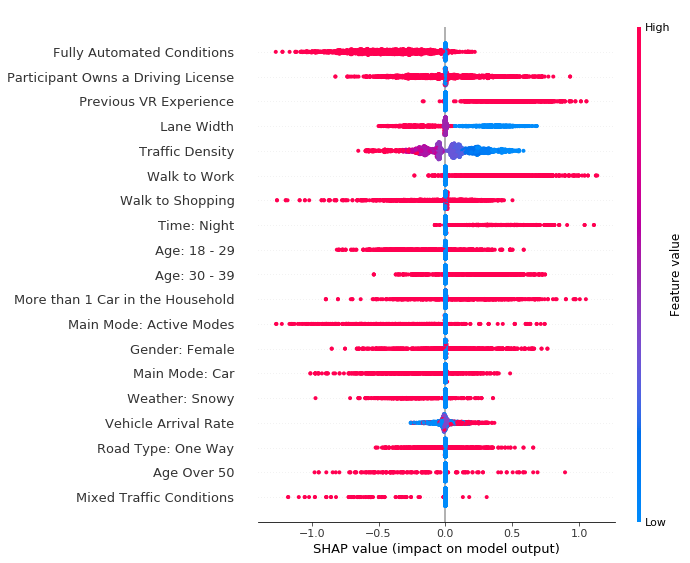
\includegraphics[scale=0.5]{chapter_4/figures/shap.png}
    \caption{Plot summary of the effects of all the covariates based on the SHAP Values}
    \label{fig:shap}
\end{figure}

\newpage